\documentclass{beamer}


\usetheme{AnnArbor}
\usecolortheme{default}


\title{Test Title}                    %TODO: Add a title.
%\subtitle{Complex Systems Engineering}
\author{Steve Mazza}
\institute[Naval Postgraduate School]
{ 
    Naval Postgraduate School \\
    Monterey, CA \\
    
\includegraphics[height=3cm]{images/NPS_logo.jpg}
}
\date {SE4940, Spring/2014}
\subject{Complex Systems Engineering}


\begin{document}

\frame{\titlepage}


%TODO: Insert content here.

%TODO: Delete everything below here to the final frame.
\frame{{Example of columns 1}
    \begin{columns}[c]      % the "c" option specifies center vertical alignment
    \column{.5\textwidth}   % column designated by a command
     Contents of the first column
    \column{.5\textwidth}
     Contents split \\ into two lines
    \end{columns}
}
 
\frame{{Example of columns 2}
    \begin{columns}[t]      % contents are top vertically aligned
    \begin{column}[T]{5cm}  % each column can also be its own environment
        Contents of first column \\ split into two lines
    \end{column}
    \begin{column}[T]{5cm}  % alternative top-align that's better for graphics 
        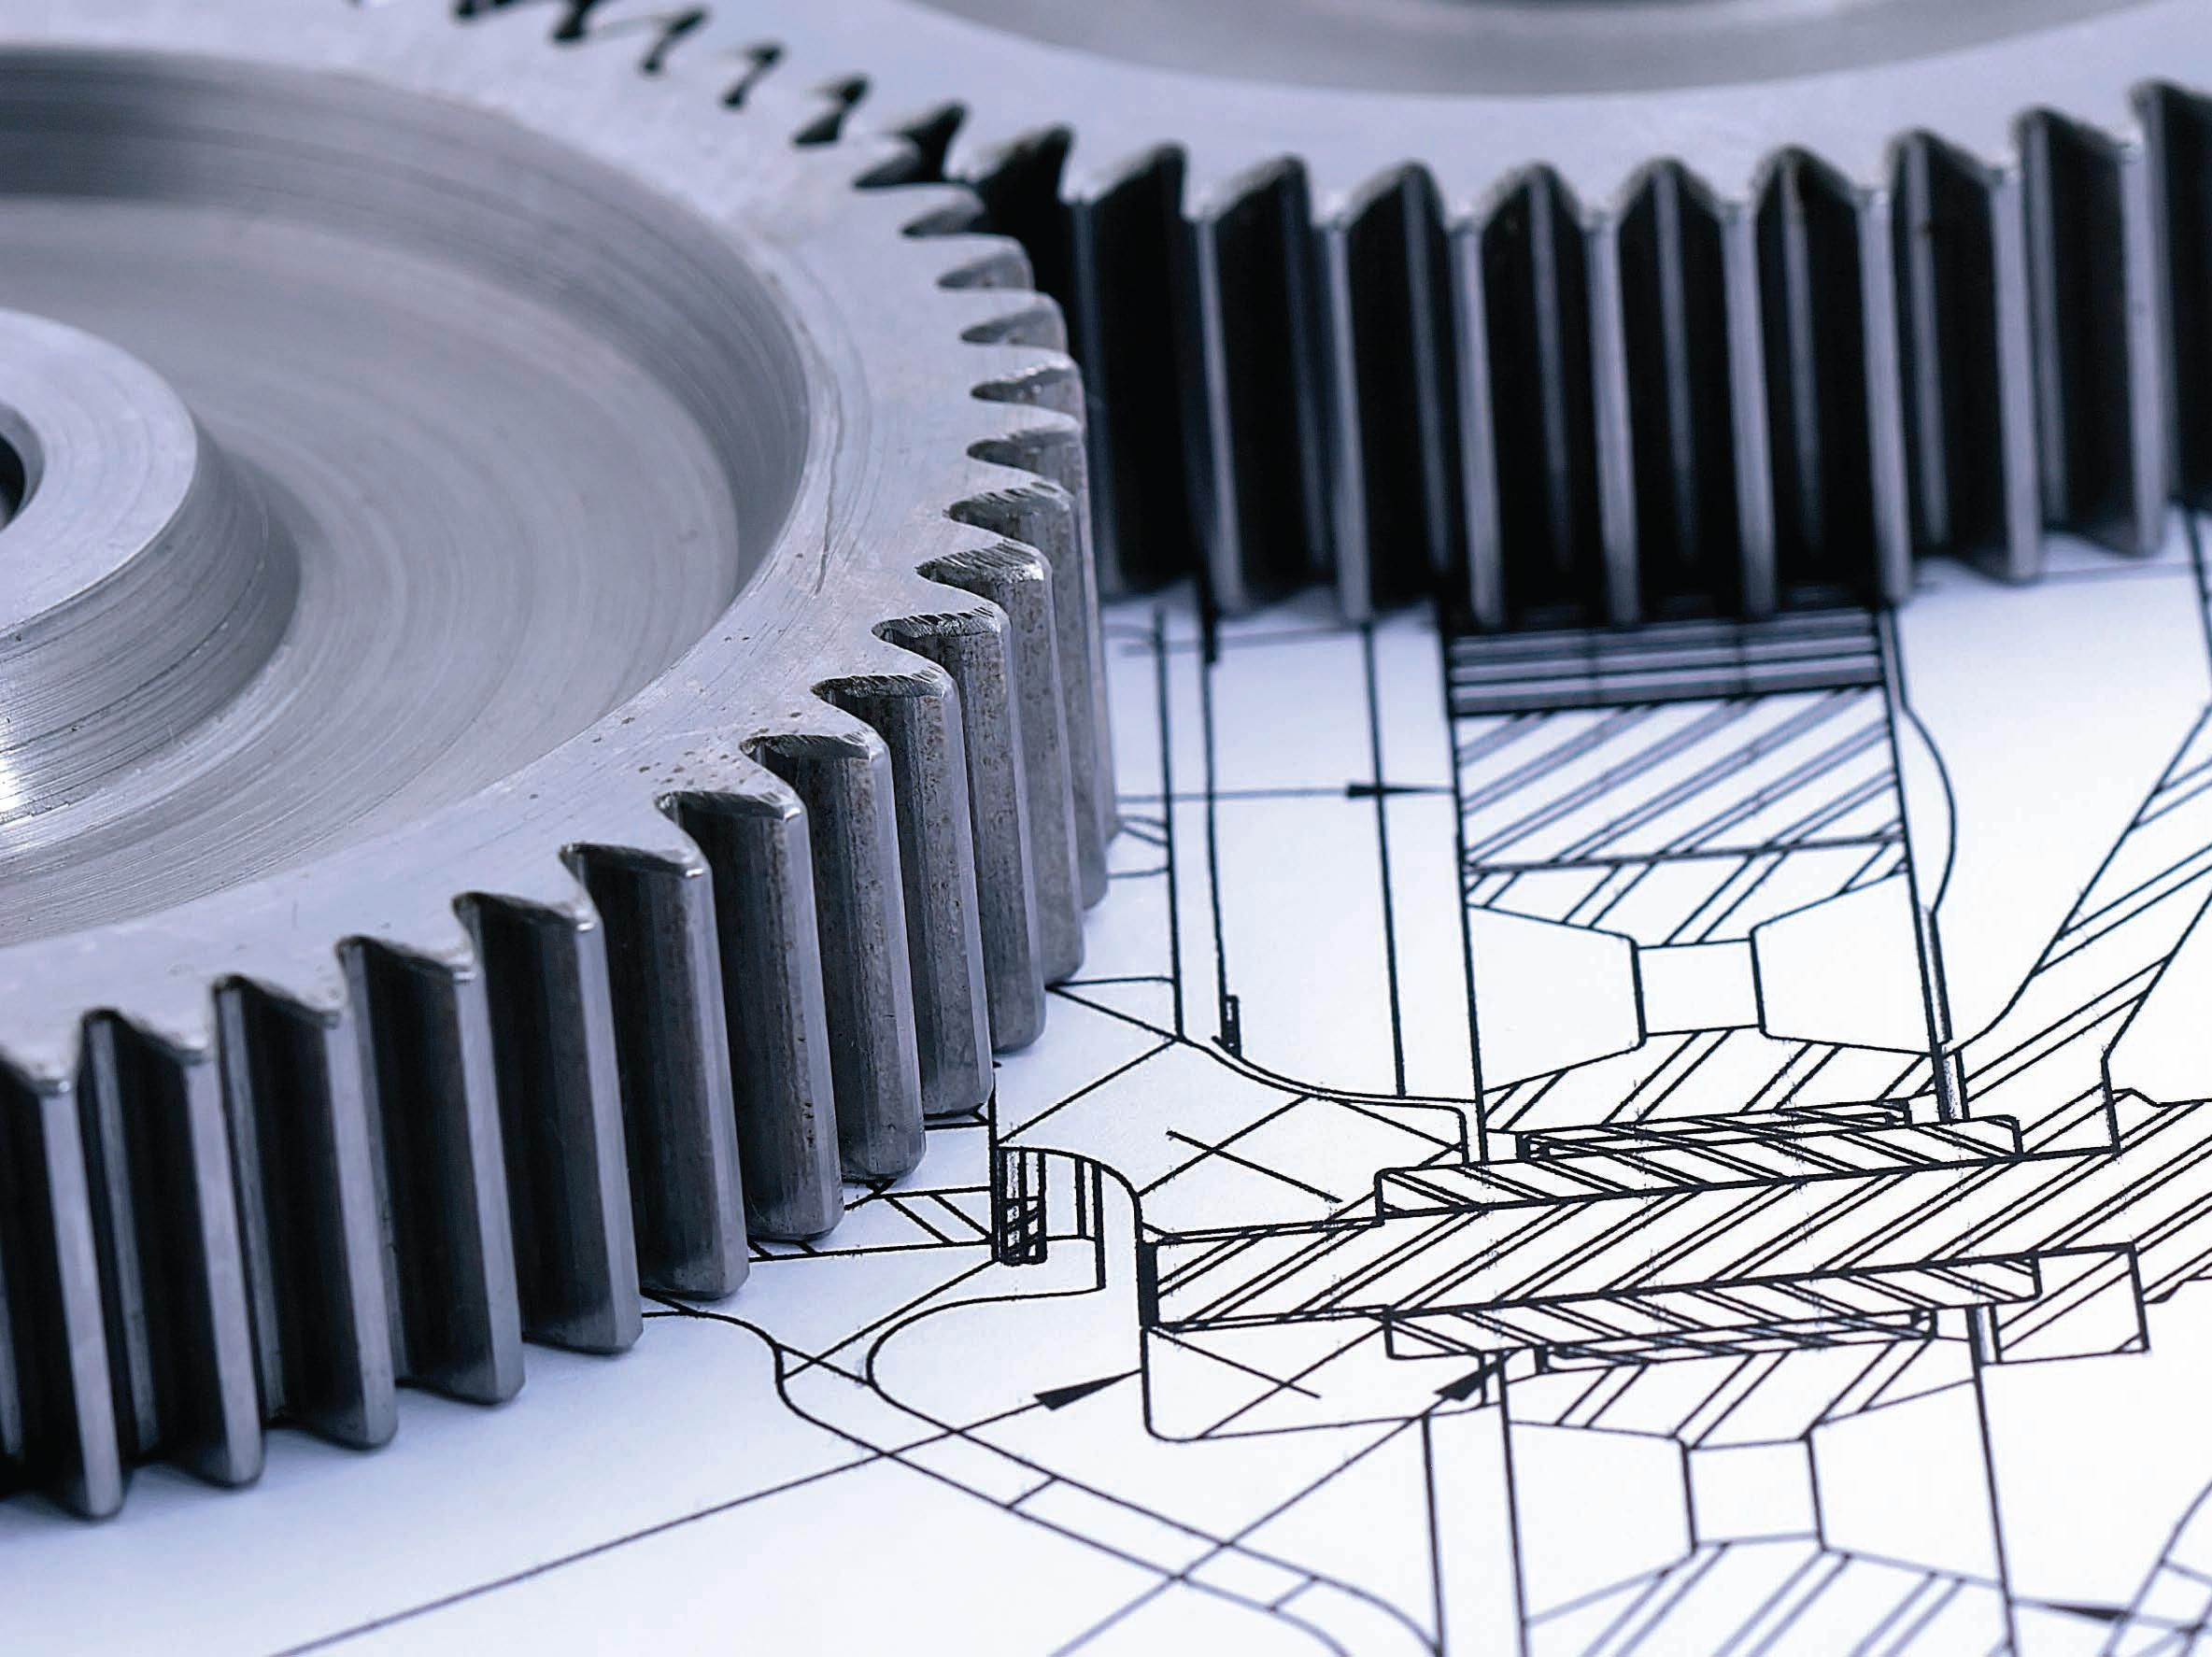
\includegraphics[height=3cm]{images/engineering.jpg}
    \end{column}
    \end{columns}
}

\frame{{Block Types}
    \begin{block}{This is a Block}
        This is important information
    \end{block}
 
    \begin{alertblock}{This is an Alert block}
        This is an important alert
    \end{alertblock}
 
    \begin{exampleblock}{This is an Example block}
        This is an example 
    \end{exampleblock}
}

\frame{{Questions?}
	\begin{center}
		
\includegraphics[width=.7\textwidth]{images/fin.png}
	\end{center}
}

\end{document}
